\documentclass{beamer}
\usepackage{listings}
\lstset{
%language=C,
frame=single, 
breaklines=true,
columns=fullflexible
}
\usepackage{subcaption}
\usepackage{url}
\usepackage{tikz}
\usepackage{graphicx}
\usepackage{tkz-euclide} % loads  TikZ and tkz-base
%\usetkzobj{all}
\usetikzlibrary{calc,math}
\usepackage{float}
\newcommand\norm[1]{\left\lVert#1\right\rVert}
\renewcommand{\vec}[1]{\mathbf{#1}}
\newcommand{\R}{\mathbb{R}}
\newcommand{\C}{\mathbb{C}}
\providecommand{\brak}[1]{\ensuremath{\left(#1\right)}}
\providecommand{\abs}[1]{\vert#1\vert}
\providecommand{\fourier}{\overset{\mathcal{F}}{ \rightleftharpoons}}
\providecommand{\pr}[1]{\ensuremath{\Pr\left(#1\right)}}
\providecommand{\sbrak}[1]{\ensuremath{{}\left[#1\right]}}
\usepackage[export]{adjustbox}
\usepackage[utf8]{inputenc}
\usepackage{amsmath}
\usetheme{Boadilla}

\graphicspath{ {figures/} }

\title{Research Paper Presentation}
\institute{IITH}
\date{CS20BTECH11054}
\author{Vaddamani Saketh}

\begin{document}
\begin{frame}
\titlepage
\end{frame}
\section{Title and Authors}
\begin{frame}
\frametitle{Title and Authors}
\begin{block}{Title}
Maximizing the Probability of Message Delivery over Ever-changing Communication Scenarios in Tactical Networks

\end{block}
\begin{block}{Authors}
\begin{itemize}
    \item Johannes F. Loevenich
    \item Roberto Rigolin F. Lopes
    \item Paulo H. Rettore
    \item Sharath M. Eswarappa
    \item Peter Sevenich
\end{itemize}

\end{block}
\end{frame}
\section{\textbf{Introduction}}
\subsection*{Prerequisites}
\begin{frame}[fragile]
\frametitle{Index Words}
\begin{block}{}
\begin{itemize}
    \item \textbf{Ever-changing Communication scenarios}: Randomly changing communication scenarios.  
    \item \textbf{message delivery}: It refers whether a message, which sender sends reaches receiver or not. 
    \item \textbf{system robustness}: It refers to the ability of tolerating perturbations that might affect the system’s functional body. In the same line robustness can be defined as "the ability of a system to resist change without adapting its initial stable configuration".
    \item \textbf{tactical networks}:  Tactical networks support military operations providing the means for network-centric warfare, among military units in large areas, through heterogeneous networks combining different communication technologies, such as High Frequency (HF), Ultra High Frequency (UHF), Very High Frequency (VHF) and Satellite Communications (SatCom).
\end{itemize}
\end{block}
\end{frame}
\subsection*{Prerequisites}
\begin{frame}[fragile]
\frametitle{}
\begin{block}{Prerequisites}
\begin{itemize}
    \item Stochastic Model
    \item Markov Chains 
    \item Node
    \item Link
    \item IP packets
\end{itemize}
\end{block}
\end{frame}
\begin{frame}[fragile]
\begin{block}{Stochastic Model}
\begin{itemize}
    \item A stochastic model represents a situation where uncertainty is present. In other words, it’s a model for a process that has some kind of randomness. These models will likely produce different results every time the model is run.
    \item In this model,probabilities are assigned to events within the model and these probabilities can be used to make predictions or supply other relevant information about the process.
\end{itemize}
\end{block}
\begin{block}{Markov Chains}
\begin{itemize}
    \item A Markov chain is a stochastic model describing a sequence of possible events in which the probability of each event depends only on the state attained in the previous event.
    \item A Markov chain is called homogeneous, if and only if the transition probabilities are independent of time t, i.e., there exist $P_{i,j}$ such that the below equation holds for all times
    \begin{align}
        P_{i,j} = \pr{X_{t}=j|X_{t-1}=i} \label{Eq:1}
    \end{align}
\end{itemize}
\end{block}
\end{frame}
\begin{frame}{}
\begin{block}{Node}
In telecommunications networks, a node is either a redistribution point or a communication endpoint.A physical network node is an electronic device that is attached to a network, and is capable of creating, receiving, or transmitting information over a communication channel.
\end{block}
\begin{block}{Link}
In a telecommunications network, a link is a communication channel that connects two or more devices for the purpose of data transmission. The link may be a dedicated physical link or a virtual circuit that uses one or more physical links or shares a physical link with other telecommunications links.
\end{block}
\begin{block}{IP packets}
In telecommunications and computer networking, a network packet is a formatted unit of data carried by a packet-switched network. A packet consists of control information and user data, also known as the payload. Control information provides data for delivering the payload.
\end{block}
\end{frame}
\begin{frame}[fragile]{Notations}
     \begin{figure}
 \centering{
    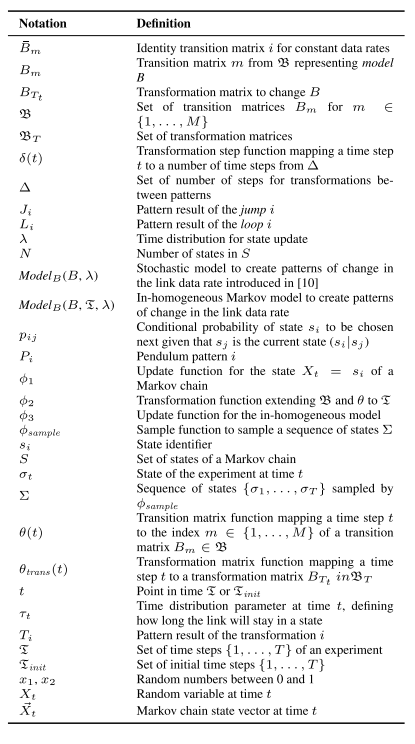
\includegraphics[width=4.5cm]{research-paper-image -6.PNG}}
    \label{Notations}
\end{figure}  
\end{frame}
\subsection*{Abstract}
\begin{frame}[fragile]
\frametitle{Abstract}
\begin{block}{Abstract}
\begin{itemize}
    \item From its earliest days, the Army has moved through doctrine, training, and equipping the forces relying on some form of networked communications. For the most part this was an Army Signal Corps function satisfied by switches, radios, satellites, and cable. 
    \item Therefore, tactical networks were crucial in their communication and they had to make sure that information being passed should not be affected by ever changing communication scenarios.
   \item So, they wanted to add an optimum redundancy to make sure that user data-flow should not be affected by packet loss, during changes in link data rate, including disconnections.
   \item Thus, we are going to introduce a stochastic model to maximize the probability of message delivery over ever-changing communication scenarios in tactical networks, implementing store-and-forward mechanisms organized in a hierarchy of layers for messages,IP packets and radios.
\end{itemize}
\end{block}
\end{frame}
\section{\textbf{Ever-changing communication scenarios}}
\subsection*{Structure of Modern Tactical Systems}
\begin{frame}[fragile]
\frametitle{}
\begin{block}{Structure of Modern Tactical Systems}
\begin{itemize}
    \item Modern tactical systems are organized into layers through multi-layer control mechanisms to handle independent changes from both user data-flows (A) and network conditions (B).
    \item  Each node has a control plane (c) and two chains: one for incoming (i) data-flows and another for outgoing (o) data-flows, both sitting in at least four layers, namely radio (0), packet (1), message (2) and proxy/broker (3)
    \item The sequence of messages from (A) enter the system from layer 3 carrying a set of QoS requirements(differentiated at layer 2), which are partially mapped to IP packets at layer 1.
    \item The radio (layer 0) usually has a buffer with limited size that differentiates the packets by priority. Note that a multi-homed node with r radio networks will have r instances of this hierarchy of queues to handle the difference in both coverage and link data rate from military communication technologies
\end{itemize}
\end{block}
\end{frame}
\begin{frame}[fragile]
\frametitle{Ever-changing end-to-end communication scenario}
\begin{figure}
    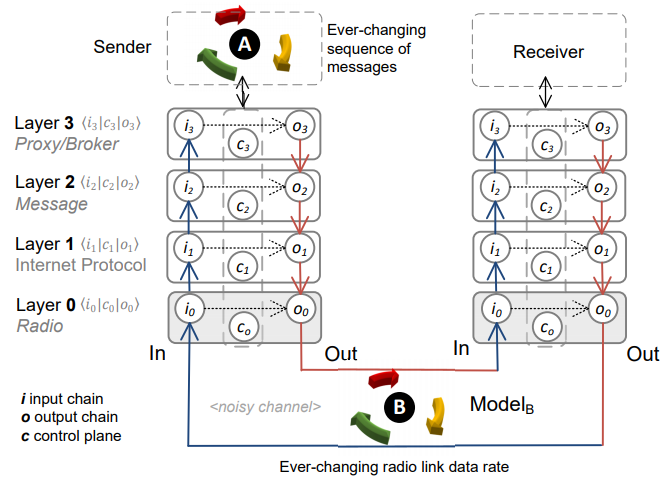
\includegraphics[scale=0.69]{research-paper-image.PNG}
    \caption{Modern tactical system model}
\end{figure}

\end{frame}
\section{Computing Probability of Message delivery}
\subsection*{Computing Probability}
\begin{frame}[fragile]
\frametitle{}
\begin{block}{Probability of Message delivery}
\begin{itemize}
    \item Let us assume that the network conditions in a communication scenario C is described as the five-tuple $C= (\overrightarrow{X_0},\beta,\theta,\beta_T,\tau)$.
    where,
    \item where $\overrightarrow{X_0}$ is the initial state vector,$\beta$ is a set of matrices describing M different probability distributions, $\theta$ is the update function, $\beta_T$ is a set of transition matrices and $\tau$ is the time distribution of the in-homogeneous Markov model, called $Model_B$
    \item This stochastic model is composed of two nested Markov chains,one representing the link data rate changes and another one defining the distributions of the pattern of data rate changes$(\beta)$.
    \item Our system implements an error correction technique called Reed Solomon Code, meaning that if the message consists of k packets and $n-k$ redundant packets, the message can be successfully delivered if at least k packets are delivered by sending a selective acknowledgement, which indicates the sequence numbers of the lost packets
\end{itemize}
\end{block}
\end{frame}
\begin{frame}[fragile]
\frametitle{Computing Probability}
Assuming independent errors that might cause packet loss,
the probability for the receiver getting any $0 \leq k \leq n$ out of
n sent packets is given by the binomial distribution as defined
in \eqref{Eq:2}.
\begin{align}
    f_X(n;p_0;k) = \pr{X = k} = {n \choose k} . p_0^{k} . (1-p_0)^{n-k} \label{Eq:2}
\end{align}
Where $p_0$ is the probability that a single packet will be delivered and X is a random variable measuring the number of successfully transmitted packets.
\end{frame}
\begin{frame}[fragile]
\frametitle{Computing Probability(contd.)}
   If $E_1$ is the event $X \geq k$, meaning that the message can be successfully delivered in the first round and $E_2$ is the event that the outer Markov chain of $Model_B$ is in state $s(t) = P_i$, we get
   \begin{align} 
      \pr{E_1|E_2} = \pr{X \geq k | s(t) = P_i} = \frac{\pr{X \geq k,s(t) = P_i}}{\pr{s(t) = P_i}} \label{Eq:3}
   \end{align}
   This construction can be extended to compute the probability $p_2$ of message delivery, during a communication scenario C consisting of I different patterns $P_1 \cup ... \cup P_i \cup ... \cup P_I = C$ by finding an optimum configuration for
   \begin{align}
       p_2 = F_{X|C}(n;p_0;k) = \pr{X \geq k} = \sum_{i=1}^{I} \pr{X \geq k_i| P_i}  \label{Eq:4}
   \end{align}
   Where the constraint $\sum_{i=1}^{I} k_i = k $ is also fulfilled at the same time.
\end{frame}
\begin{frame}[fragile]
\frametitle{}
\begin{block}{Probability of packet delivery within a Time window}
\begin{itemize}
    \item We assume that the data rate changes of the system follow an in-homogeneous Markov chain represented by $Model_B$ with state space $\beta = B_1, . . . , B_M$ resulting in a communication scenario C.
    \item We also assume that the distributions $B_1, . . . , B_m$ together with the distribution $\lambda$ are well-known and therefore we have access to an oracle knowing the link states $\Sigma = [b(1), . . . , b(T)]$ at each point in time $t \in \tau = [1, . . . , T]$.
    \item We define the function $f_l(t) = [max(0, \sum_{i=1}^{t-1} \tau_i - 1), \sum_{i=1}^{t-1} \tau_i - 1)]$ mapping a point in time $t \in \tau$ to a time interval describing how many seconds the link (inner Markov chain) stays in state $b(t) \in [0,1,2,3,4,5]$.
\end{itemize}
\end{block}
\end{frame}
\begin{frame}[fragile]
\frametitle{Probability of packet delivery within a Time window(contd.)}
Assuming the probability of delivering a packet $p_0(T_w)$ is proportional to the amount of bits received within the time window $T_{w} = f_{l}(t_1) \cup f_{l}(t_2)$ and the packet size is distributed by $\kappa$, the optimal data rate $b_{opt}(t)$ for almost sure delivery can be calculated using the ratio
\begin{align}
b_{opt}(T_w) = \frac{\kappa}{\abs{T_w}} \label{Eq:5}
\end{align}
we can now compute the ratio between the current data rate $b(t)$ and the optimal data rate $b_{opt}(t)$ for arbitrary time windows $T_w$.
\begin{align}
b_{ratio} = \frac{\sum_{t=t_1}^{t_2} \frac{f_l(t)}{\abs{T_w}}b(t)}{b_{opt}(T_w)} \label{Eq:6}
\end{align}
\end{frame}
\begin{frame}[fragile]
\frametitle{Probability of packet delivery within a Time window(contd.)}
So, now we can use $b_{ratio}$ to introduce another function $g(t, b(t), b_{opt}(T_w))$ that computes an initial guess for the probability of packet loss at layer 0.

\begin{block}{}
\begin{align}
  g(T_w, b(t), b_{opt}(T_w)) =  \begin{cases}
			0, & \text{if} b(t) = 0 \forall t \in [t_1,t_2] \\
            b_{ratio}, & \text{if}  \sum_{t=t_1}^{t_2} \frac{f_l(t)}{\abs{T_w}}b(t) < b_{opt}(T_w) \\
            1, & \text{if}  \sum_{t=t_1}^{t_2} \frac{f_l(t)}{\abs{T_w}}b(t) \geq b_{opt}(T_w)
		 \end{cases}  \label{Eq:7}
\end{align}
\end{block}
\end{frame}
\begin{frame}[fragile]
\frametitle{}
\begin{block}{Interpretation of function g}
\begin{itemize}
    \item If $g = 0$, then there is only one possibility which is $b(t)$ is zero for the entire time period $T_w$
    \item If $g = b_{ratio}$, then we can solve the equation, either for fixed $\abs{T_w(t)}$ or b to adjust the system parameters such that $g=1$ and as a result $p_0(t) > 0$.
    \begin{align}
      \frac{\abs{T_w(t)}.b}{\kappa} = 1 - g(t, b(t), b_{opt}(T_w))  \label{Eq:8}
    \end{align}
    \item If $g=1$ and $b(t) = (1+\epsilon).b_{opt}(t)$, then we can increase the probability of packet delivery $p_0(t)$ by adding redundancy $r(t) = \epsilon.b_{opt}(t)$ . Where, $\epsilon = (b(t) - b_{opt}(t)) / b_{opt}(t)$
    \item From the above analysis of g, we can say that 
\end{itemize}
\begin{align}
    p_0(T_w) = \pr{X = 1|b(t), T_w, \kappa} \label{Eq:9}
\end{align}
\end{block}
\end{frame}
\section{Maximising the Probability of message delivery}
\subsection*{Maximising the Probability of message delivery}
\begin{frame}[fragile]
\frametitle{Maximising Probability of Message delivery}
 Let $F_{X|C}(n=r+k;p_0;k)$ be the objective function describing the binomial distribution, in \eqref{Eq:4}, of successful message delivery given communication scenario C and the number of data packets k, find the optimum amount of redundancy r s.t.
\begin{align}
  \mathop{max}_{r} F_{X|C}(n=r+k;p_0;k) & = \mathop{min}_{r} 1 - F_{X|C}(n=r+k;p_0;k) \notag \\
  & = \mathop{min}_{r} 1 - \sum_{i=1}^{I} f_{X|P_i}(n_i=r_i+k_i;p_0;k_i) \label{Eq:10}
\end{align}
Where, constraints are:
\begin{align}
    \sum_{i=1}^{I} k_i = k; \hspace{10}\sum_{i=1}^{I} r_i = r; \hspace{10} n_i - k_i \geq 0;   \hspace{10} r_i,n_i,k_i \geq 0; \label{Eq:11}
\end{align}
\end{frame}
\subsection{Algorithm to find optimum amount of redundancy}
\begin{frame}[fragile]
\frametitle{Algorithm to find optimum amount of redundancy}
\begin{figure}
    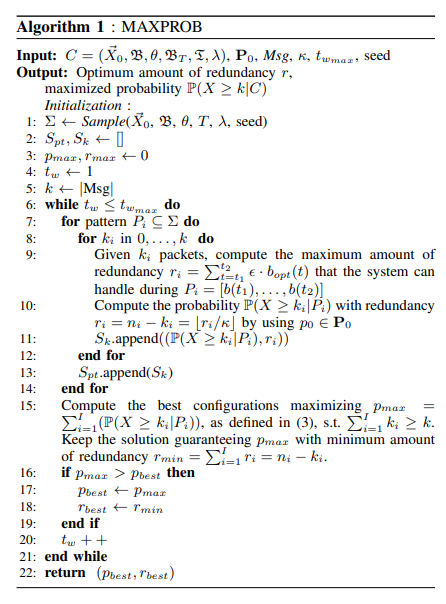
\includegraphics[scale=0.55]{research-paper-image -2.PNG}
    \caption{MAXPROB Algorithm}
\end{figure}
\end{frame}
\begin{frame}[fragile]
\frametitle{Theorem to prove an algorithm exists to find optimum solution}
\begin{block}{Theorem}
Given a non-empty, ever-changing communication scenario $C= (\overrightarrow{X_0},\beta,\theta,\beta_T,\tau)$, the probabilities $P_0$ for different end-to-end delays 1, . . . , $t_{w_{max}}$ over stable system conditions, the number $k > 0$ of data packets defining the length of a message Msg, the distribution of the the packet size $\kappa$ and the maximum end-to-end delay $t_{w_{max}}$ , MAXPROB computes an optimum amount of redundancy.
\end{block}
\end{frame}
\begin{frame}[fragile]
\frametitle{Proof for the theorem}
\begin{block}{Proof}
We will be proving inductively that for each possible end-to-end
delay $1 \leq t_w \leq t_{w_{max}}$, $p_{best}$ is always maximized by the
optimal amount of redundancy $r_{best}$.

Let $t_w = 1$, then lines 7-12 compute the maximum redundancy $r_i$ and the corresponding probability $\pr{X \geq k_i|P_i}$ by using the probabilities $p_0 \in P_0$ for each possible combination of a pattern $P_i$ and number of packets $k_i \leq k$. The probabilities
for fixed pattern Pi are stored in the data structure $S_k$ and added to $S_{pt}$ afterwards.In sequence (line 15), the algorithm computes all possible configurations by maximizing $p_2$ from \eqref{Eq:3}.We keep the configuration that uses a minimum amount of redundancy $r_{min}$.Since $p_{max} > p_{best}$ is true, we update $p_{best}$ and $r_{best}$.Thus, By line 15 $r_{best}$ is an optimal configuration for $t_w = 1$ with probability. \\
The induction step $(t_{w}) \implies (t_{w} + 1)$ can be done in the same way. Since $p_{best}$ and $r_{best}$ are only updated if the algorithm finds a higher probability $p_{max}$, the tuple $r_{best}$ is always an optimal solution. Hence, Proved.
\end{block}
\end{frame}
\begin{frame}[fragile]
\frametitle{Multi-layer Stochastic Uncertainty Model}
Given the probabilities $p_{i}(T_{w})$, $i \in Layers[0, 2]$, We assume that M is an instance of $Model_B$ and that we are given the 5-tuple $C= (\overrightarrow{X_0},\beta,\theta,\beta_T,\tau)$ required to sample the sequence Σ by computing $\phi_{sample}$.
Now we can define two functions to convert the instance M to an instance U of an stochastic model describing the uncertainty of the underlying tactical system by replacing the system states of the inner Markov chain of M by probabilities $p_0$ and the pattern $P_j$ representing the states of the outer Markov chain by $p_2$.To this end, we define the function $\psi_{in}$ mapping each system
state to a probability $p_0$ as
\begin{align}
    \psi_{in} : (s_{in}(t),t) \implies (\pr{X=1|b(t)=s_{in}(t),T_w=f_l(t),\kappa)} \label{Eq:12}
\end{align}

We can fix the state of the outer Markov
chain for a time interval $[t_1, t_2]$ with $0 \leq t_{1},t_{2} \leq T$, meaning that the system follows a pattern $P_j = [s_{in}(t1), . . . , s_{in}(t2)]$ generated by single matrix $B_j \in \beta$. Given size k of a message, we can now replace $P_j$ by maximized probability $p_2$ using $\psi_{out}$
\begin{align}
    \psi_{out} : (P_j,t_1,t_2,k) \implies \pr{X \geq k|P_i = P_j,T_w = f_l(t_1) \cup f_l(t_2), \kappa} \label{Eq:13}
\end{align}

\end{frame}
\begin{frame}[fragile]
\section{Experimental Results}
\frametitle{}
\begin{block}{Experimental Results}
\begin{itemize}
    \item We used two loop patterns, L1 and L2, and the VHF network. Both patterns of change include very low link data rates (i.e 0.6 and 1.2 kbps) and even link disconnections (0 kbps) resulting in packet loss. 
    \item Here, we demonstrate how redundancy can improve the message/packet delivery over the loop patterns L1  and L2, both with 200 states updated every 10 seconds. The messages were composed by 1, 3, 9, 18 and 54 packets, and the sender packet rate was distributed according to (0.05, 0.075, 0.1, 0.2, 0.5, 1, 2) packet/second.
    \item The below figure complements the results from this table by showing the probability for message delivery as a function of different time windows $T_{w}$ for six messages sizes, namely 1, 3, 9, 18 and 54 packets per message. In this figure, there are two examples representing 100$\%$ (left) and 200$\%$ (right) for L1.showing that the probabilities converge with respect to the size of the maximum end-to-end delay $T_{w}$; also called time window.
\end{itemize}
\end{block}
\end{frame}
\begin{frame}[fragile]
\frametitle{Experimental Results}
\begin{figure}
    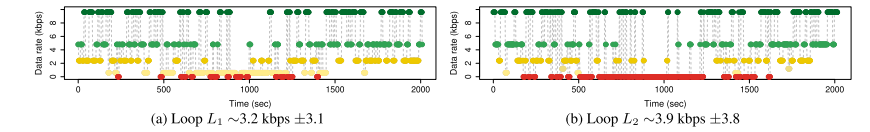
\includegraphics[scale=0.5]{research-paper-image -5.PNG}
    \caption{Loops L1 and L2}
\end{figure}
\begin{figure}
    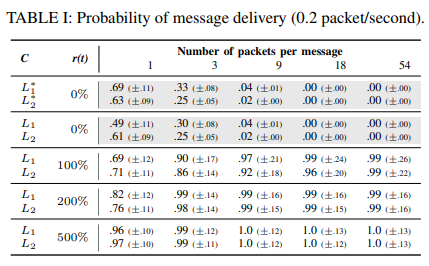
\includegraphics[scale=0.33]{research-paper-image -3.PNG}
    \caption{Probability of message delivery(0.2 packet/second).}
\end{figure}
\begin{figure}
    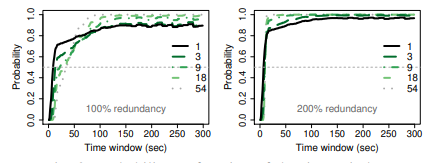
\includegraphics[scale=0.5]{research-paper-image -4.PNG}
    \caption{Probability as a function of the time window.}
\end{figure}
\end{frame}
\begin{frame}[fragile]
\frametitle{}
\begin{block}{Conclusion}
\begin{itemize}
    \item This paper introduced a stochastic model to maximize the probability of message/packet delivery using the hierarchy of layers from modern tactical systems.
    \item The goal was to estimate the optimum redundancy level to mitigate packet loss in communication scenarios with link disconnection therefore increasing the probability of delivering messages. Thus, we started with the hypothesis that transport protocols can use our model to proactively add redundancy to reduce the packet loss observed during radio link disconnections.
    \item Our hypothesis was verified with experiments sending messages with different sizes through a VHF link with data rate changing in two different patterns. The experimental results suggest that our stochastic model can compute close to optimal parameters for a transport protocol using redundancy to overcome packet loss during link disconnections, also avoiding data overhead from packet acknowledgements and packet re-transmissions.
\end{itemize}
\end{block}
\end{frame}

\begin{frame}[fragile]
   \centering
    \textcolor{blue}{\Huge{\textbf{THANK YOU}}}
 \begin{figure}
 \centering{
    
\includegraphics[width=3cm]{logo.png}}
    \label{logo}
\end{figure}  
\end{frame}

\end{document}